\appendix

\newgeometry{total={210mm,297mm},left=30mm,right=30mm,bindingoffset=5mm, top=25mm,bottom=25mm}
\begin{partwithabstract}{Appendix}
  Apendices to the document:
  \begin{enumerate}
    \item Software environment used
    \item Agreement documents for use of two datasets.
  \end{enumerate}
\end{partwithabstract}
\restoregeometry

\chapter{Train test split detail\label{sec:appendix_split}}

The datasets in this research are both stratified and grouped (due to USiegen containing multiple scans from the same patient).
These were splitted in a train, validation and test set taking into account these characteristics.
This was discussed in chapter \ref{sec:trainValTestSplit} on page \pageref{sec:trainValTestSplit}.
The result of this operation is detailed in the following tables.

\begin{tabular}{llll}
\toprule
{} &           patient &           scan\_id &  split \\
\midrule
0   &  MyoSegmenTUM\_001 &  MyoSegmenTUM\_001 &  train \\
1   &  MyoSegmenTUM\_002 &  MyoSegmenTUM\_002 &   test \\
2   &  MyoSegmenTUM\_003 &  MyoSegmenTUM\_003 &  train \\
3   &  MyoSegmenTUM\_004 &  MyoSegmenTUM\_004 &  train \\
4   &  MyoSegmenTUM\_005 &  MyoSegmenTUM\_005 &   xval \\
5   &  MyoSegmenTUM\_006 &  MyoSegmenTUM\_006 &   test \\
6   &  MyoSegmenTUM\_007 &  MyoSegmenTUM\_007 &  train \\
7   &  MyoSegmenTUM\_008 &  MyoSegmenTUM\_008 &  train \\
8   &  MyoSegmenTUM\_009 &  MyoSegmenTUM\_009 &  train \\
9   &  MyoSegmenTUM\_010 &  MyoSegmenTUM\_010 &  train \\
10  &  MyoSegmenTUM\_011 &  MyoSegmenTUM\_011 &   test \\
11  &  MyoSegmenTUM\_012 &  MyoSegmenTUM\_012 &   test \\
12  &  MyoSegmenTUM\_013 &  MyoSegmenTUM\_013 &  train \\
13  &  MyoSegmenTUM\_014 &  MyoSegmenTUM\_014 &  train \\
14  &  MyoSegmenTUM\_015 &  MyoSegmenTUM\_015 &  train \\
15  &  MyoSegmenTUM\_016 &  MyoSegmenTUM\_016 &   xval \\
16  &  MyoSegmenTUM\_017 &  MyoSegmenTUM\_017 &  train \\
17  &  MyoSegmenTUM\_018 &  MyoSegmenTUM\_018 &  train \\
18  &  MyoSegmenTUM\_019 &  MyoSegmenTUM\_019 &   xval \\
19  &  MyoSegmenTUM\_020 &  MyoSegmenTUM\_020 &  train \\
20  &  MyoSegmenTUM\_021 &  MyoSegmenTUM\_021 &  train \\
21  &  MyoSegmenTUM\_022 &  MyoSegmenTUM\_022 &   test \\
22  &  MyoSegmenTUM\_023 &  MyoSegmenTUM\_023 &  train \\
23  &  MyoSegmenTUM\_024 &  MyoSegmenTUM\_024 &   test \\
24  &  MyoSegmenTUM\_025 &  MyoSegmenTUM\_025 &  train \\
25  &  MyoSegmenTUM\_026 &  MyoSegmenTUM\_026 &  train \\
26  &  MyoSegmenTUM\_027 &  MyoSegmenTUM\_027 &  train \\
27  &  MyoSegmenTUM\_028 &  MyoSegmenTUM\_028 &   xval \\
28  &  MyoSegmenTUM\_029 &  MyoSegmenTUM\_029 &  train \\
29  &  MyoSegmenTUM\_030 &  MyoSegmenTUM\_030 &  train \\
30  &  MyoSegmenTUM\_031 &  MyoSegmenTUM\_031 &   xval \\
31  &  MyoSegmenTUM\_032 &  MyoSegmenTUM\_032 &  train \\
32  &  MyoSegmenTUM\_034 &  MyoSegmenTUM\_034 &  train \\
33  &  MyoSegmenTUM\_035 &  MyoSegmenTUM\_035 &   test \\
34  &  MyoSegmenTUM\_036 &  MyoSegmenTUM\_036 &   xval \\
35  &  MyoSegmenTUM\_037 &  MyoSegmenTUM\_037 &   xval \\
36  &  MyoSegmenTUM\_038 &  MyoSegmenTUM\_038 &  train \\
37  &  MyoSegmenTUM\_039 &  MyoSegmenTUM\_039 &  train \\
38  &  MyoSegmenTUM\_040 &  MyoSegmenTUM\_040 &  train \\
39  &  MyoSegmenTUM\_041 &  MyoSegmenTUM\_041 &  train \\
40  &  MyoSegmenTUM\_042 &  MyoSegmenTUM\_042 &  train \\
41  &  MyoSegmenTUM\_043 &  MyoSegmenTUM\_043 &   xval \\
42  &  MyoSegmenTUM\_044 &  MyoSegmenTUM\_044 &  train \\
43  &  MyoSegmenTUM\_045 &  MyoSegmenTUM\_045 &  train \\
44  &  MyoSegmenTUM\_046 &  MyoSegmenTUM\_046 &  train \\
45  &  MyoSegmenTUM\_047 &  MyoSegmenTUM\_047 &  train \\
46  &  MyoSegmenTUM\_048 &  MyoSegmenTUM\_048 &  train \\
47  &  MyoSegmenTUM\_049 &  MyoSegmenTUM\_049 &   test \\
48  &  MyoSegmenTUM\_050 &  MyoSegmenTUM\_050 &  train \\
49  &  MyoSegmenTUM\_051 &  MyoSegmenTUM\_051 &   test \\
50  &  MyoSegmenTUM\_052 &  MyoSegmenTUM\_052 &   xval \\
51  &          PLoS\_001 &          PLoS\_001 &  train \\
52  &          PLoS\_002 &          PLoS\_002 &  train \\
53  &          PLoS\_003 &          PLoS\_003 &  train \\
54  &          PLoS\_004 &          PLoS\_004 &  train \\
55  &          PLoS\_005 &          PLoS\_005 &   xval \\
56  &          PLoS\_006 &          PLoS\_006 &   test \\
57  &          PLoS\_007 &          PLoS\_007 &  train \\
58  &          PLoS\_008 &          PLoS\_008 &  train \\
59  &          PLoS\_009 &          PLoS\_009 &  train \\
60  &          PLoS\_010 &          PLoS\_010 &  train \\
61  &          PLoS\_011 &          PLoS\_011 &   xval \\
62  &          PLoS\_012 &          PLoS\_012 &   test \\
63  &          PLoS\_013 &          PLoS\_013 &  train \\
64  &          PLoS\_014 &          PLoS\_014 &  train \\
65  &          PLoS\_015 &          PLoS\_015 &  train \\
66  &          PLoS\_016 &          PLoS\_016 &  train \\
67  &          PLoS\_017 &          PLoS\_017 &   xval \\
68  &          PLoS\_018 &          PLoS\_018 &   test \\
69  &          PLoS\_019 &          PLoS\_019 &  train \\
70  &          PLoS\_020 &          PLoS\_020 &  train \\
71  &          PLoS\_021 &          PLoS\_021 &   xval \\
72  &          PLoS\_022 &          PLoS\_022 &   test \\
73  &       USiegen\_001 &       USiegen\_003 &  train \\
74  &       USiegen\_001 &       USiegen\_006 &  train \\
75  &       USiegen\_001 &       USiegen\_016 &  train \\
76  &       USiegen\_002 &       USiegen\_008 &  train \\
77  &       USiegen\_002 &       USiegen\_014 &  train \\
78  &       USiegen\_002 &       USiegen\_001 &  train \\
79  &       USiegen\_002 &       USiegen\_010 &  train \\
80  &       USiegen\_002 &       USiegen\_000 &  train \\
81  &       USiegen\_004 &       USiegen\_002 &  train \\
82  &       USiegen\_007 &       USiegen\_005 &  train \\
83  &       USiegen\_007 &       USiegen\_009 &  train \\
84  &       USiegen\_008 &       USiegen\_012 &   test \\
85  &       USiegen\_009 &       USiegen\_015 &  train \\
86  &       USiegen\_010 &       USiegen\_004 &   xval \\
87  &       USiegen\_015 &       USiegen\_007 &  train \\
88  &       USiegen\_016 &       USiegen\_013 &  train \\
89  &       USiegen\_018 &       USiegen\_011 &   test \\
90  &      xVertSeg\_001 &      xVertSeg\_001 &  train \\
91  &      xVertSeg\_002 &      xVertSeg\_002 &  train \\
92  &      xVertSeg\_003 &      xVertSeg\_003 &  train \\
93  &      xVertSeg\_004 &      xVertSeg\_004 &  train \\
94  &      xVertSeg\_005 &      xVertSeg\_005 &  train \\
95  &      xVertSeg\_006 &      xVertSeg\_006 &  train \\
96  &      xVertSeg\_007 &      xVertSeg\_007 &   xval \\
97  &      xVertSeg\_008 &      xVertSeg\_008 &  train \\
98  &      xVertSeg\_009 &      xVertSeg\_009 &   xval \\
99  &      xVertSeg\_010 &      xVertSeg\_010 &  train \\
100 &      xVertSeg\_011 &      xVertSeg\_011 &   test \\
101 &      xVertSeg\_012 &      xVertSeg\_012 &  train \\
102 &      xVertSeg\_013 &      xVertSeg\_013 &  train \\
103 &      xVertSeg\_014 &      xVertSeg\_014 &   test \\
104 &      xVertSeg\_015 &      xVertSeg\_015 &   xval \\
\bottomrule
\end{tabular}



\chapter{Used software \& Reproducability of this research}

\section{Reproducability of the used environment}
The reproducability of this work has been ensured in several ways:
\begin{description}
  \item[Data]: All datasets used in this project are publically available. For some datasets, it is required to request permission, like the author of this work has done.
  \item[Software]: This project was performed completely in python, a publically available programming language. 
  All packages used are open-source.
  To reproduce this research, no software has to be purchased. 
  \item[Code]: Both code an text of this project can be found on a public GitHub repository
  \footnote{It is possible that small adaptations of the code are required to run it on other hardware. For example, to run it using a GPU with less internal memory it could be necessary to reduce the batch size.}. 
  \item[Docker]: The specific environment to run the code mentioned above can also be found in the mentioned GitHub repository in the form a dockerfile.
  It should be noted that this dockerfile requires a GPU that supports CUDA.   
\end{description}

The above mentioned aspects should allow other researchers to reproduce the results in this document.
This work makes use of parts of \textit{haven.ai} \footnote{This is a collection of libraries developed by the team of dr. I. Laradji to manage different experiments in deep learning research.} 
as a basis to manage different experiments.
These experiments are conducted using the deep learning library \textit{PyTorch}.
This tool is widely used in boty industry and academic research.
A list of other Machine Learning tools used in this work is provided below.
Table \ref{tab:UsedTools} is not an exhaustive list of all  python libraries used in this work.
It aims to list the more advanced tools, crucial for this work.

\begin{SCtable}[\sidecaptionrelwidth][h]
 
  \begin{tabular}{ p{2cm} l l } 
   \hline
   \hline
   \textbf{Library} & \textbf{version} & \textbf{reference}    \\
   \hline 
  Python & 3.8 & Programming language \\
   \hline
   \multicolumn{3}{c}{Deep learning and machine learning tools} \\
   \hline
   PyTorch & 1.7.1 & Deep learning library \\ 
   scikit-learn & 0.24.2 & Machine learning toolbox \\
   \hline
   \multicolumn{3}{c}{Tools to work with (medical) images} \\
   \hline
   SimpleITK & 2.0.2 & Library for medical images \\ 
   kornia & 0.2.0 & Computer vision library linked to torch \\
   scikit-image & 0.18.1 & Image manipulation library \\
   Pillow & 8.2.0 & Image manipulation\\
   \hline
   \multicolumn{3}{c}{Tools for matrix \& scientific computation} \\
   \hline
   numpy & 1.20.3 & matrix manipulation \\
   scipy & 1.6.3 & scientific calculation \\
   \hline
   \multicolumn{3}{c}{Result visualization} \\
   \hline
   matplotlib & 3.4.2 & data visualization \\ 
   seaborn & 0.11.1 & data visualization \\
   \multicolumn{3}{c}{Neural network experiment management} \\
   \hline
   haven & xxx & experiment management \\ 
   \hline
   \hline
  \end{tabular}
  \caption{Python libraries used. \label{tab:UsedTools}}

\end{SCtable}

Table \ref{tab:UsedTools} is not an exhaustive list of all libraries used in this work.
One can quickly dublicate the environment used in this work by building the \textit{Docker} environment defined in xxx.

\section{Hardware}
GeForce RTX 2080 Ti (4352 CUDA cores)
total memory 11264 MB
CUDA version 11.2

Intel® Core™ i7-9700 CPU @ 3.00GHz $\times$ 8 
RAM : 32 GB

\section{Other}
The formatting of this document, bringing Tufte layout elements in the \LaTeX memoir class, is based on the excelent post found on \url{https://tex.stackexchange.com/questions/275565/tufte-layout-in-painless-memoir}.
The Neural network architecture illustrations xxx were made using this project: \url{https://github.com/HarisIqbal88/PlotNeuralNet}.
The conceptual illustration of the neural network idea on page xxx is based on xxx.



\newgeometry{total={210mm,297mm},left=30mm,right=30mm,bindingoffset=5mm, top=25mm,bottom=25mm}
\chapter{Dataset agreements\label{seg:datasetagreement}}

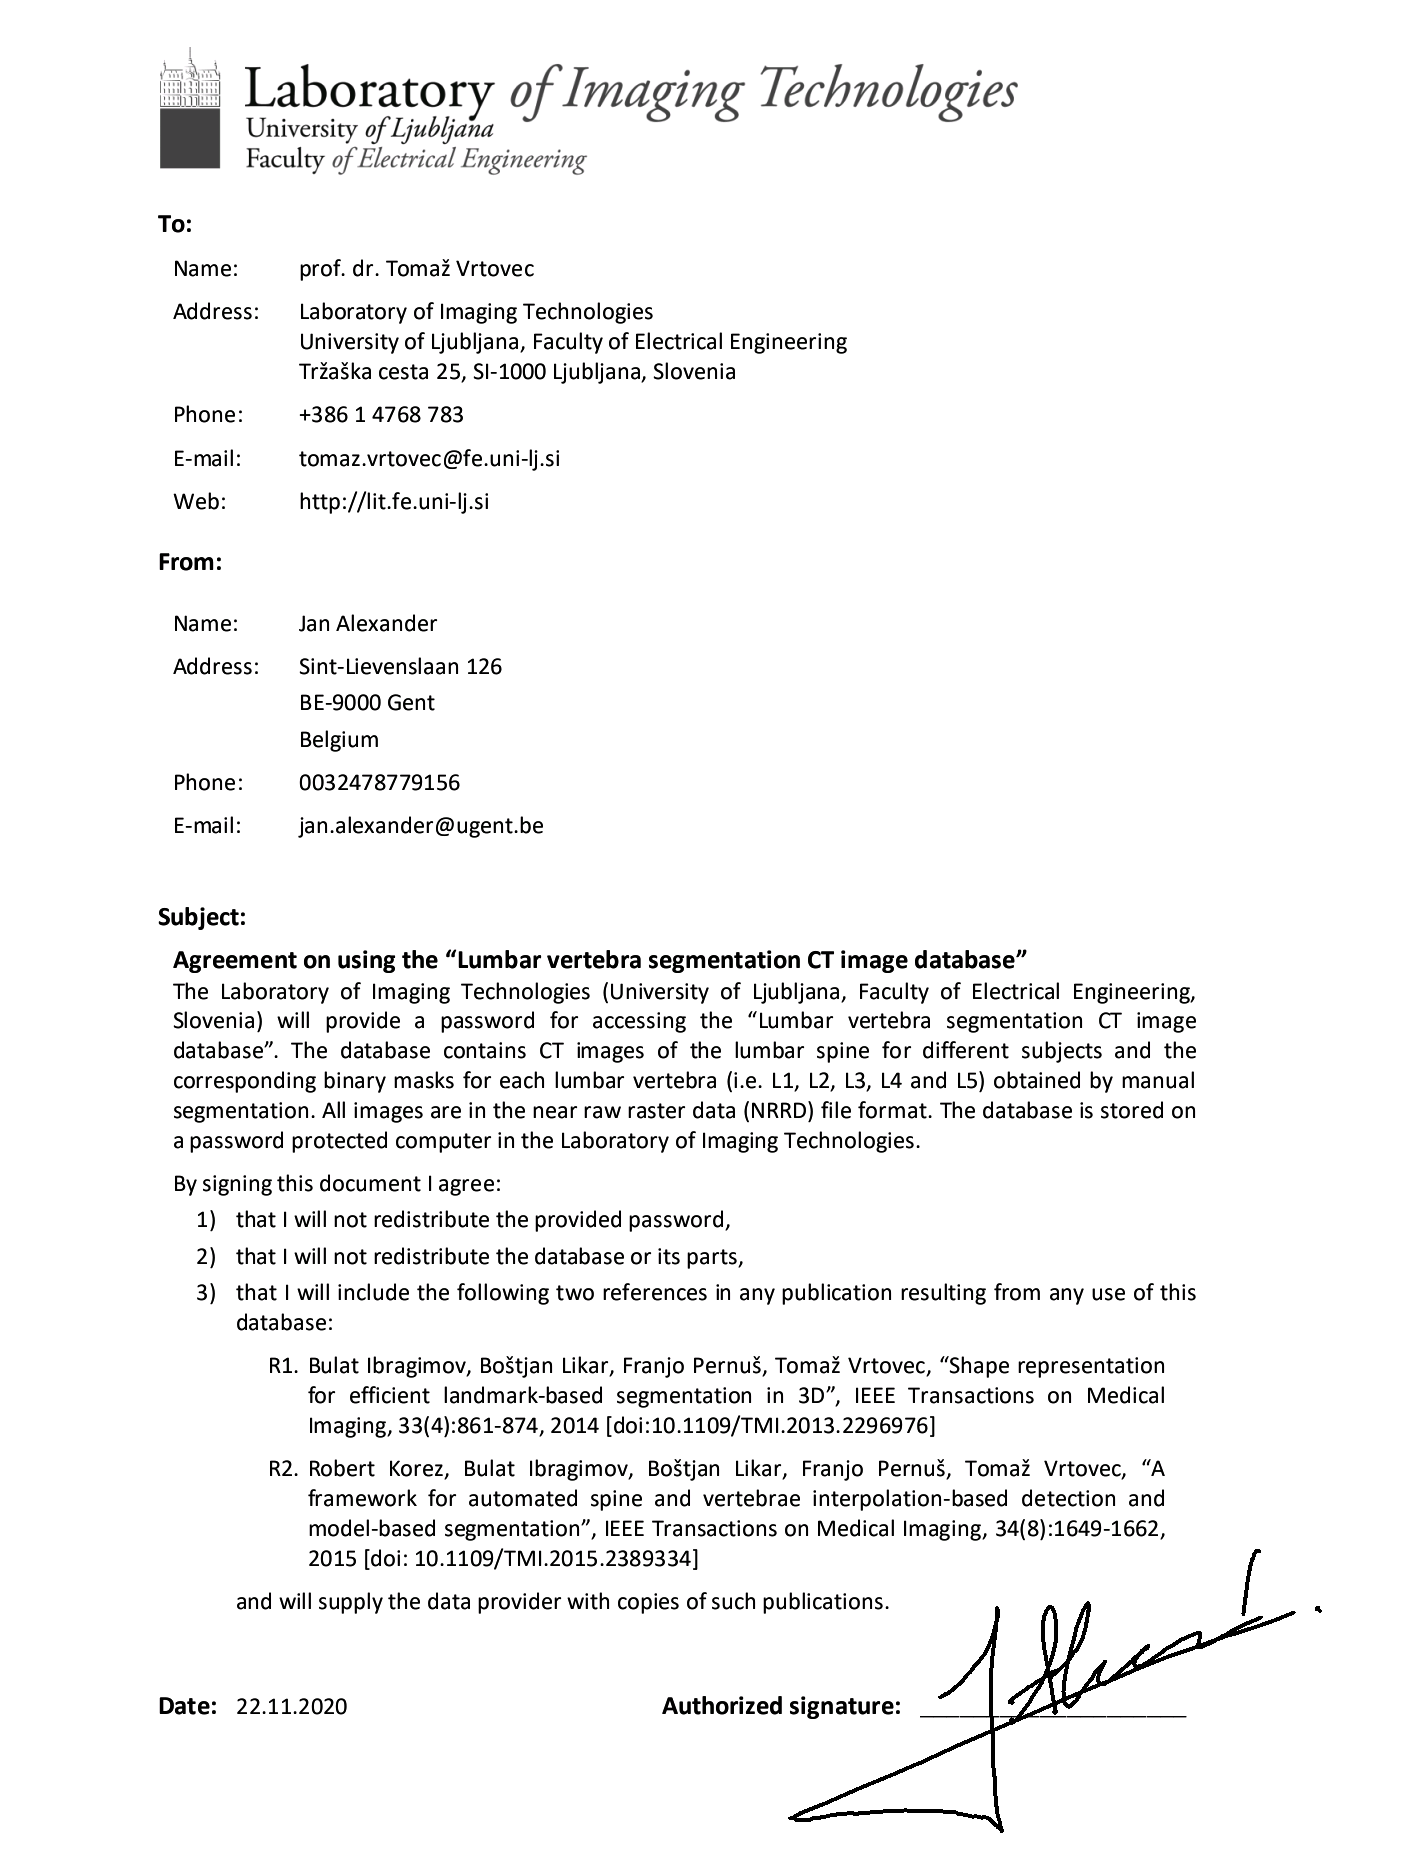
\includegraphics[width=17cm]{/home/thesis/images/AgreementxVertSeg.png}

\chapter{Predefence and seminars}
\par{
  On March 31$^st$, 2021 the concept of this work was presented in a poster session seated by Prof. Stijn Vansteelandt.
The poster used during this event is included on the next page for reference.
}




\includepdf[fitpaper=true, pages=-]{/home/thesis/images/Addendum_thesis_seminars.pdf}
\includepdf[fitpaper=true, pages=-]{/home/thesis/images/Poster_JanAlexander.pdf}
